\documentclass{beamer}

\author{AJ Fagan}
\title{Network Synergy Project Intro}
\date{October 4, 2024}

\usepackage{graphicx}
\graphicspath{ { ./figs } }

\usetheme{Madrid}
\usecolortheme{beaver}

\begin{document}

\frame{\titlepage}


\begin{frame}
  \frametitle{Table of Contents}
  \tableofcontents
\end{frame}

\section{Drug Synergy}

\begin{frame}
  \frametitle{Synergy via Potency}
  Just a simple visualization of Bliss Synergy.
\end{frame}

\begin{frame}
  \frametitle{Promises of Synergistic Combinations}
  \begin{itemize}
    \item Overcoming chemoresistance 
    \item Repurposing existing drugs
    \item Increasing efficacy
    \item Reducing toxicity
  \end{itemize}

  And then I do the bit where I say that potency synergy only actually enables consideration of the first 3.    
\end{frame}

\begin{frame}
  \frametitle{Relevant XKCD}
  XKCD comic about killing cancer cells with a handgun.

  Other avenues are needed to more accurately predict clinical benefits of drug combinations in early in vitro experiments.
\end{frame}


\section{Network Synergy}

\begin{frame}
  \frametitle{Synergy via Biological Networks}
  Consider the effects of drugs on a biological network, such as a GRN.

  Image of a network.

  Enables qualitative assessment of drug interaction.
\end{frame}

\begin{frame}
  \frametitle{Module Approach}
  \begin{figure}[!htb]
    \minipage{0.4\textwidth}
      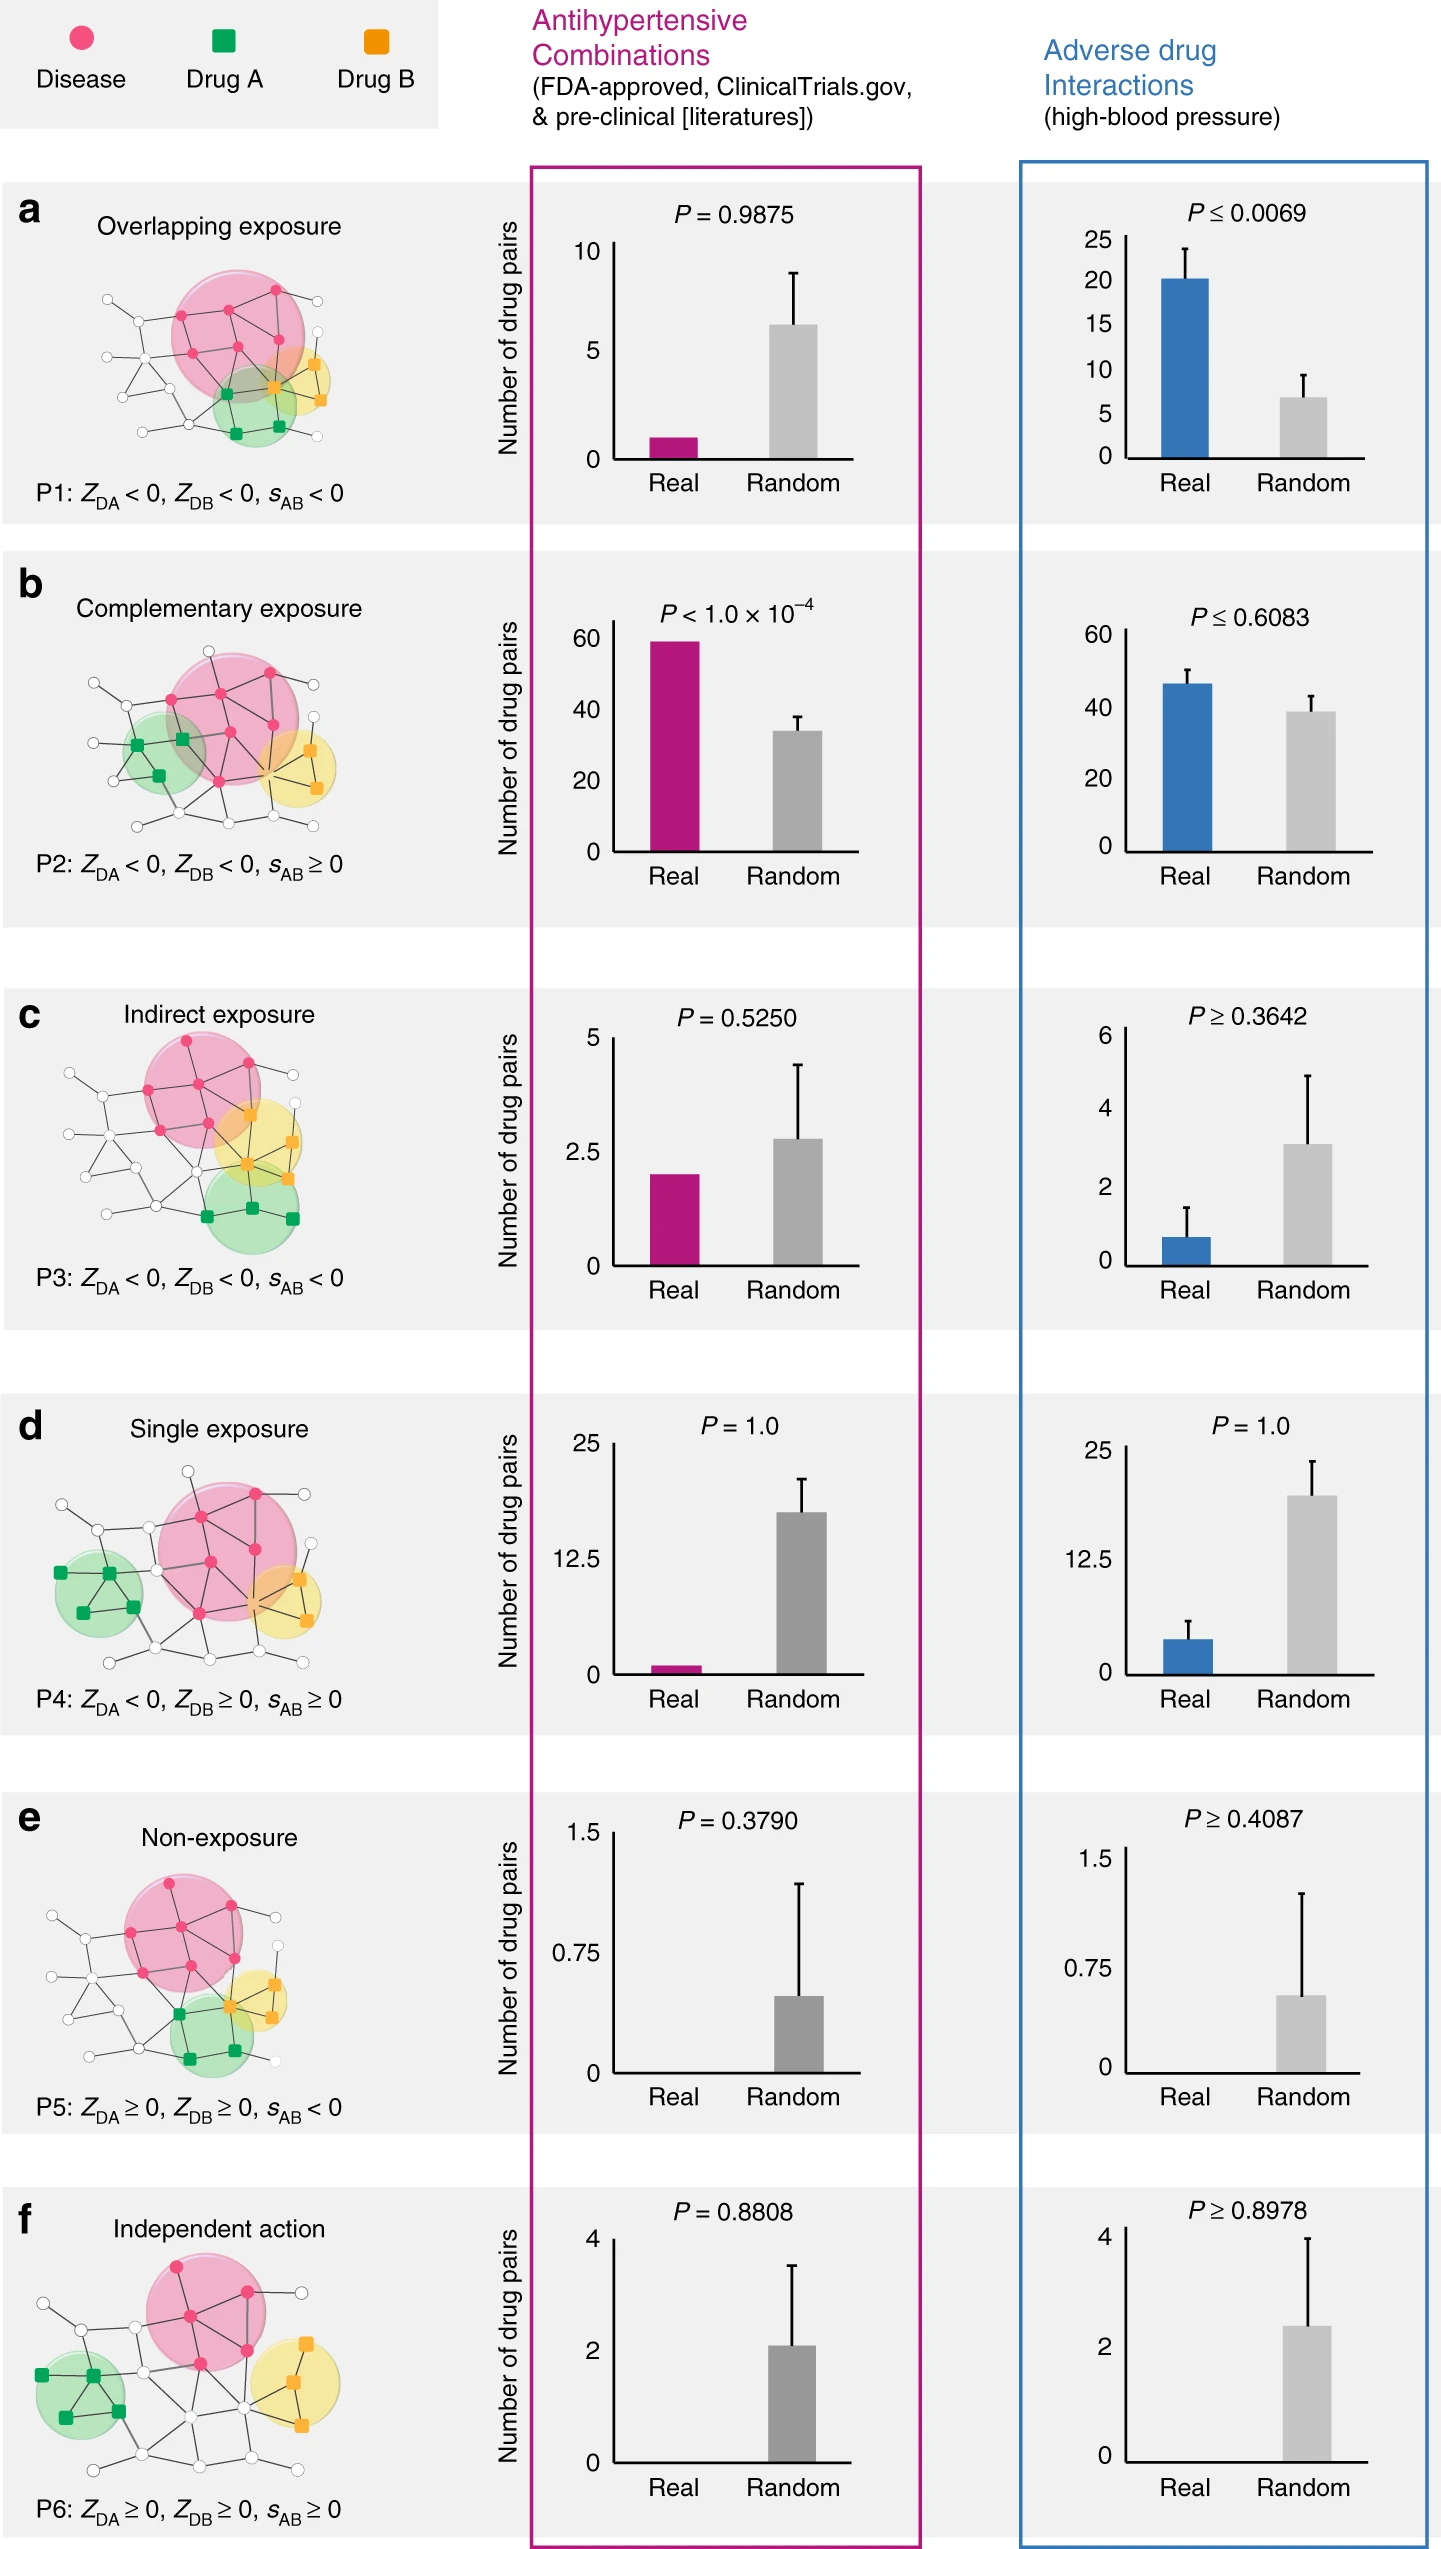
\includegraphics[width=\linewidth, height=200]{figs/barabasi-hypertension}
    \endminipage
    \minipage{0.4\textwidth}
      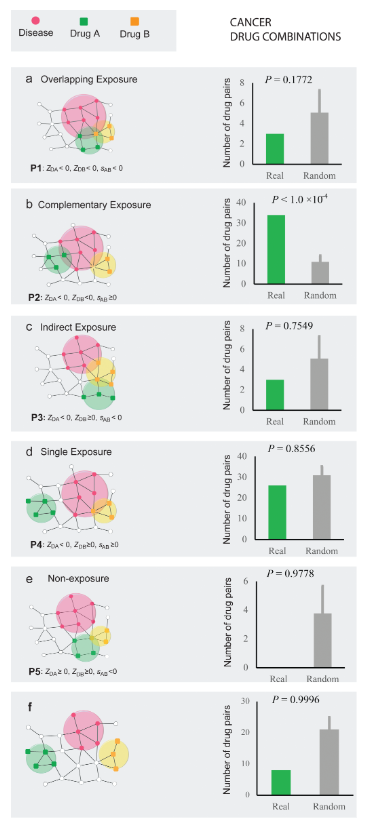
\includegraphics[width=\linewidth, height=200]{figs/barabasi-cancer.png}
    \endminipage
  \end{figure}
\end{frame}

\begin{frame}
  \frametitle{Module Approach - Further Directions}
  The Barabasi paper only really discusses efficacy of the principles via approved drug combinations --- biased.
  \vfill
  Try to expand on this method by:
  \begin{itemize}
      \item Performing network analysis of drug combinations (0, A, B, AB) in various principles.
      \item Considering \underline{T}umor \underline{M}icro\underline{e}nvironments (TMEs).
      \item Similarity scores were reduced to binary $\geq0$ or $<0$ --- do smaller/larger similarity scores make a difference?
  \end{itemize}
\end{frame}

\begin{frame}
  \frametitle{Quantitative Approach}

  Apply the concepts of Potency Synergy onto biological networks.

  \begin{itemize}
    \item Which genes/proteins/metabolites are over/under-active in the combination, relative to what we would expect from the monotherapies?
    \item GSEA $\Rightarrow$ Which cell functions are over/under-active?
  \end{itemize}

  \vfill

  Does this method provide any benefit over the Module Approach? What is the drug module of AB --- is it greater than A $\cup$ B?
\end{frame}

\section{Tumor Microenvironments}

\begin{frame}
  \frametitle{Network Synergy in TMEs}
  Cancer cells are not the only part of the tissue that contribute to cancer activity.

  Reinclude fig from "Module Approach"

  TMEs may expand and specialize the disease module into modules $D_1, \ldots D_K$. 
  What network principles do we see with these TME modules?
\end{frame}

\begin{frame}
  \frametitle{Multiplex Implantable Microdevice Assay}
  (This is the Joe Gray paper)

  Utilizes spatial analysis of the TME to predict efficacious combinations of targeted/chemotherapeutic drugs with immunotherapy.

  \vfill

  "multiplex immunostaining and imaging process that measures the expression levels of $>30$ different protein markers in each cell. Computational analysis of the resulting multiplex images provided information about drug-induced changes in the compositions, functional states and organizations of the tumor and TME cells. These measurements provided mechanistic insights that were used to select drug combinations that were predicted to be effective when administered systemically. These combinations included targeting treatment-resistant cancer stem cells."
  
  \vfill
  
  Never mentions networks. What principles are exhibited in these data? 
\end{frame}

\section{Prediction of in vivo efficacy}

\begin{frame}
  \frametitle{Predicting in vivo efficacy}
  More generally, the goal of this project is to develop a metric that is:
  \begin{itemize}
    \item Inexpensive to obtain
    \item Simple to calculate
    \item Predictive of \textit{in vivo} outcomes
  \end{itemize}

  As a result, would likely need either to conduct \textit{in vivo} (e.g. murine) studies, or try to utilize existing data. 
\end{frame}

\end{document}
